\chapter{Client Application Architecture}

\section{Overview}
The client application of Project Zoom is a web-based application. It can be run using a HTML5-capable web browser. The client application accesses the server's resources through a REST interface. The code is partitioned into several modules. An architectural pattern similar to Model-View-Controller (MVC) is applied.

\subsection{MV* pattern family}
The Model-View-Controller (MVC) pattern was first introduced by Reenskaug in 1979 \cite{Reenskaug_1979} and later published by Krasner et al. in 1988 \cite{Krasner_1988}. It was one of the first approaches to separate business and presentation logic code within a software project.

\begin{figure}
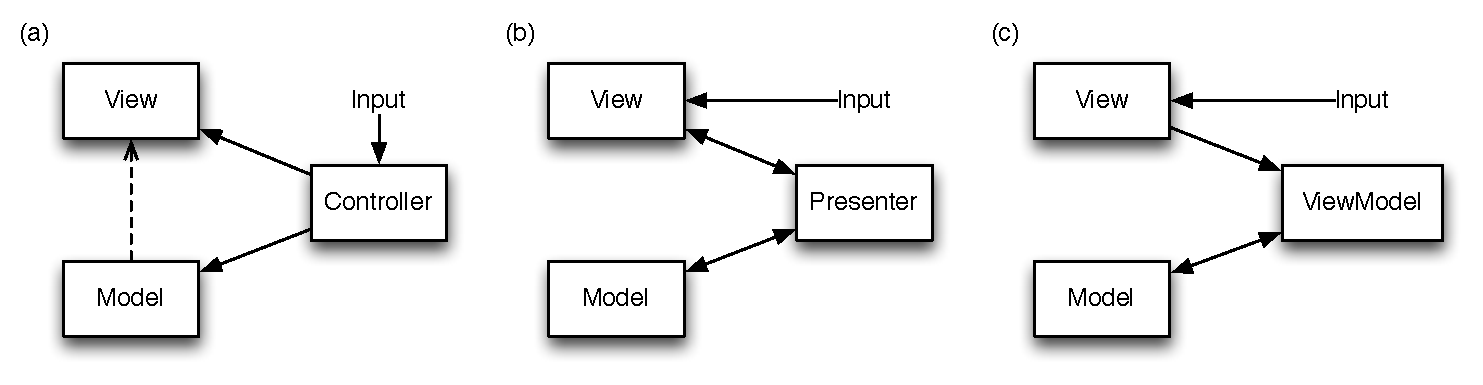
\includegraphics[width=\textwidth]{mvc-mvp-mvvm.pdf}
\caption[Diagrams of Model-View-Controller, Model-View-Presenter and Model-View-ViewModel]{\textit{(a)} Model-View-Controller \textit{(b)} Model-View-Presenter \textit{(c)} Model-View-ViewModel}
\label{fig:MV}
\end{figure}

A \textbf{Model} is an active representation of the data in the system. It usually encapsulates methods for fetching, persisting and transforming the data. It also emits events upon data changes that Controllers and Views can listen to. The Model itself is ignorant of any particular user interface. A \textbf{View} encapsulates all the code required to display a user interface with the data from the Model. A \textbf{Controller} is responsible for updating the Model when a user manipulates the View. \cite{Krasner_1988} \cite{Gamma_1994}

Since its introduction in the 1980's the MVC has mutated to accommodate modern technologies. The architectural patterns MVC, Model-View-Presenter (MVP) and Model-View-ViewModel (MVVM) as shown in figure \ref{fig:MV} a–c are commonly referred to as the MV* pattern family \cite{Osmani_2012}. Because of the separation of business and presentation logic MV* patterns are widely used in the development of web applications \cite{Takada_2012}.

Model-View-Presenter (MVP) is derived from MVC to achieve a complete separation between Model and View. Whereas in MVC the View depends on the Model in MVP the View is agnostic to a specific Model and can be reused for different Models. The Presenter replaces the Controller and has the responsibility to connect the interfaces of Model and View. 

Model-View-ViewModel (MVVM) is based on the concepts of MVP. However, the Presenter is replaced by a ViewModel, which contains a subset of the Model as well as additional state and methods. The ViewModel and the View communicate through data-binding\footnote{Data-binding is technique where properties of a Model can be assigned to user interface components in a way that changes from either are reflected to the other. \cite{Bent_2004}} and events. Because Model and View are separated the ViewModel connects both and contains logic in state-change and event handlers.

MVP and MVVM are commonly used in scenarios where it is important to have user interface components that are general-purpose and have to be reused in several different locations. Such applications are usually enterprise or consumer application with a large number of Views. MVC is a more lightweight approach, which is well suited for applications with a smaller number of Views and conceptual tight coupling between presentation and data. \cite{Osmani_2012}

The client application of Project Zoom only has a few Views, as described in section \ref{sec:design}. The interactive graph (see: use case \ref{uc:organize} and \ref{uc:versions}) is a very close representation of the respective Model. Also, it has to be custom developed as there are no applicable standard components available. Based on these observations the MVC architecture has been selected for the client application of Project Zoom. Figure \ref{fig:arch} shows the implemented architecture. The shown components are detailed in later sections.

\begin{figure}
\missingfigure{Architecture diagram}
\caption{Architecture diagram}
\label{fig:arch}
\end{figure}


\subsection{Event-driven programming}
\label{sec:eventbased}

Users expect computer systems to respond quickly. This is especially true for web applications \cite{Selvidge_1999}. In any case users expect the interface to be non-blocking when the system is performing long running tasks \cite{Nielsen_1994}.  In web applications this is achieved through asynchronous APIs for tasks like requesting data from the server \footnote{XMLHttpRequest, \url{http://www.w3.org/TR/XMLHttpRequest/}, accessed 06/19/13} or waiting for user input \footnote{Document Object Model Events, \url{http://www.w3.org/TR/DOM-Level-3-Events/}, accessed 06/19/13}. An event-driven system is a popular solution for dealing with asynchronous code execution \cite{Michelson_2006}. 

\textbf{Events} are messages sent between components in a system. The receiver has to subscribe a type of events, which senders then eventually publish (see: Observer pattern \cite{Gamma_1994}). There are two categories of events:
\begin{itemize}
\item Global events are only idenitfied by their names and can be received by any object in the system.
\item Object specific events are identified by both their names and sender objects. Receivers need to have a reference to the sending object when subscribing for this kind of events.
\end{itemize}

Event-driven programming is a concept where components of a system heavily communicate by events. Particularly, data changes and user actions are propagated using events. Using an event-driven approach leads to looser coupling between components. Thus, producing better testable and maintainable code \cite{Faison_2011}.

Requesting data from the server (see: use case \ref{uc:fromhome}), waiting for user inputs and listening for data synchronization messages (see: requirement \ref{req:concurrency}) are asynchronous tasks that the Project Zoom client performs. Using an event-driven architecture allows the system to pass data streams efficiently through the system.

\subsection{Synchronization}
As a collaborative web application, Project Zoom allows multiple users to access and manipulate shared resources (see: requirement \ref{req:concurrency}). There are four popular approaches for dealing with synchronization issues in distributed systems: locking, event-passing, three-way merges and differential synchronization \cite{Fraser_2009}.

\begin{figure}[!h]
\begin{center}
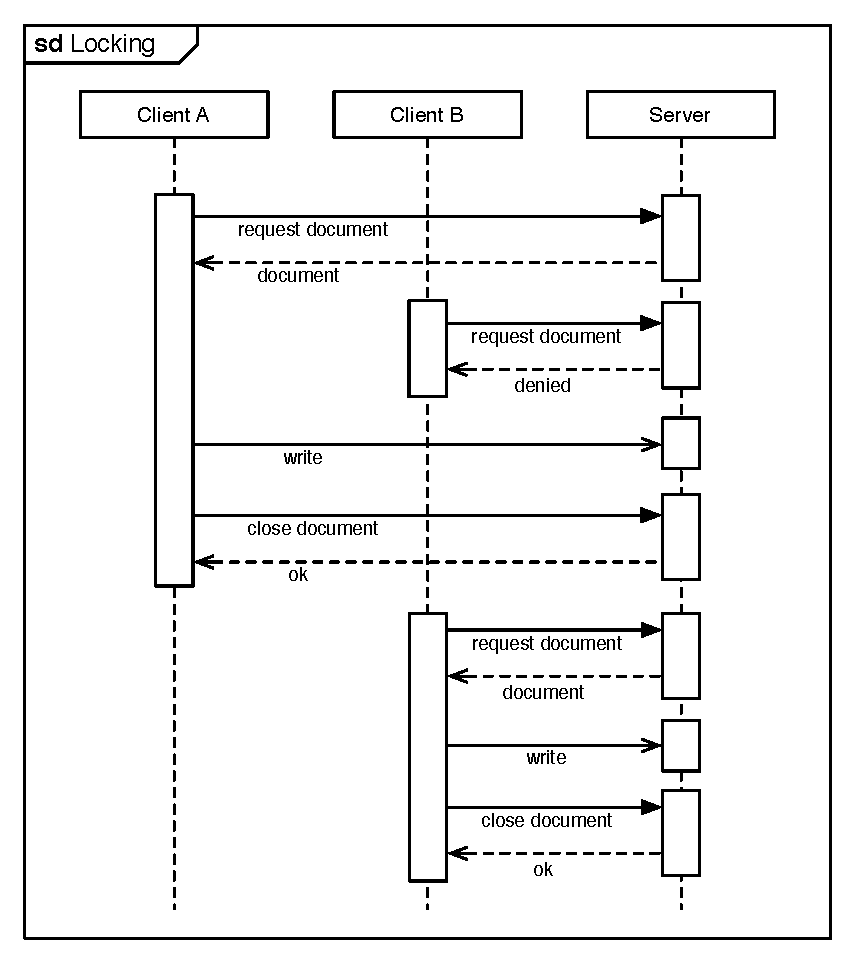
\includegraphics[width=0.5\textwidth]{locking_seq.pdf}
\caption{Sequence diagram of synchronization with locking}
\label{fig:locking}
\end{center}
\end{figure}

\textbf{Locking} is a mechanism to enforce mutual exclusion and is a standard solution to synchronization \cite{Dijkstra_1965}. Figure \ref{fig:locking} outlines how locking ensures consistency as only one user has access to the resource at a time. Due to its ensured consistency locking is implemented in a variety of applications, e.g. ACID\footnote{Atomicity, Consistency, Isolation and Durability (ACID) are a set of properties that database transactions guarantee. \cite{Gray_1981}}-compliant database systems, office applications\footnote{File locking in Microsoft Word, \url{http://support.microsoft.com/default.aspx?scid=kb;EN-US;176313}, accessed 06/25/13} and Document-collaboration software\footnote{MediaWiki Documentation: LockManager, \url{https://doc.wikimedia.org/mediawiki-core/master/php/html/classLockManager.html}, accessed 06/25/13}. As realtime collaboration\footnote{Realtime collaboration is a mechansim where the changes to a document on a client are immediately propagated to the other clients. Because of network-latency, the realtime property is in this context not as narrow as in the fields of operating systems or computer graphics. \cite{Sun_2002}} systems require concurrent access to shared resources, locking is not suitable for this class of systems.

\begin{figure}[!h]
\begin{center}
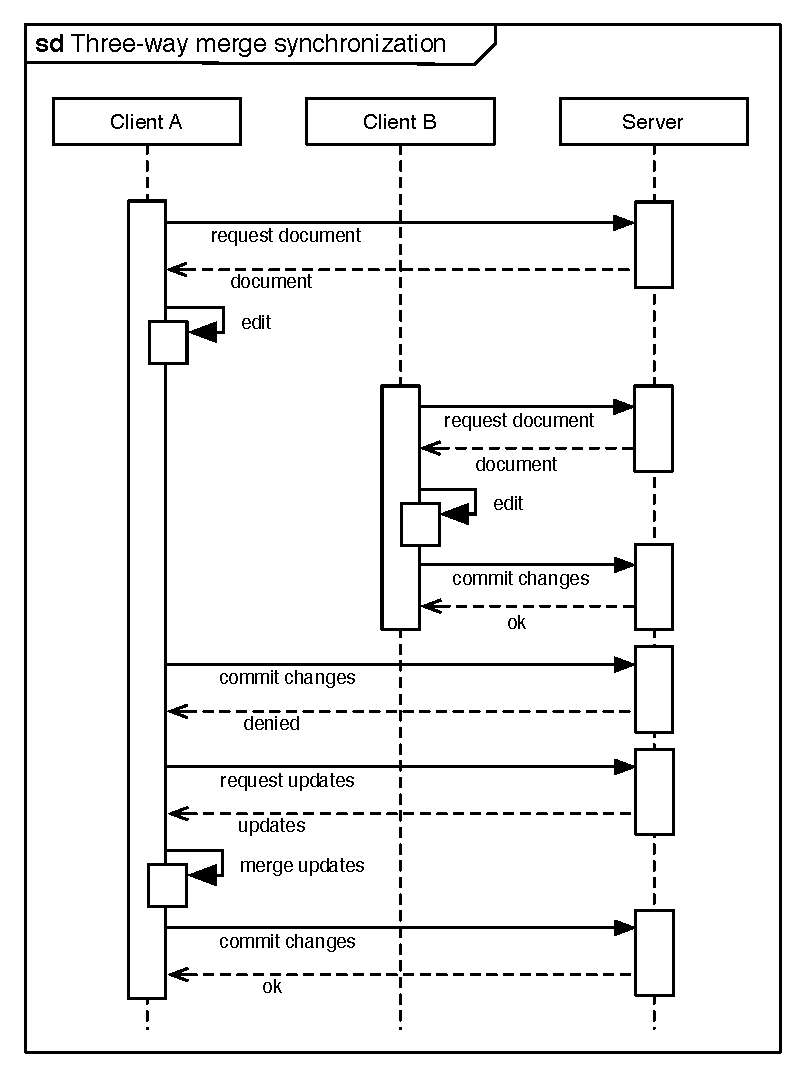
\includegraphics[width=0.5\textwidth]{threeway_seq.pdf}
\caption{Sequence diagram of three-way merge synchronization}
\label{fig:threeway}
\end{center}
\end{figure}

The \textbf{three-way merge} is a synchronization approach that has been implemented in some revision control systems \cite{Pilato_2008}. As shown in figure \ref{fig:threeway}, the clients hold a local version of a document and make edits to it individually. When synchronizing these changes, the client first requests updates from the server and merges them locally. Then the synchronized data is sent to the server. A system using the three-way merge approach is not guaranteed to be consistent as synchronization is only triggered when a client publishes an edit. This edit is not automatically propagated to other collaborating clients. Therefore, this approach is not suitable for realtime collaboration systems, either.

\begin{figure}[!h]
\begin{center}
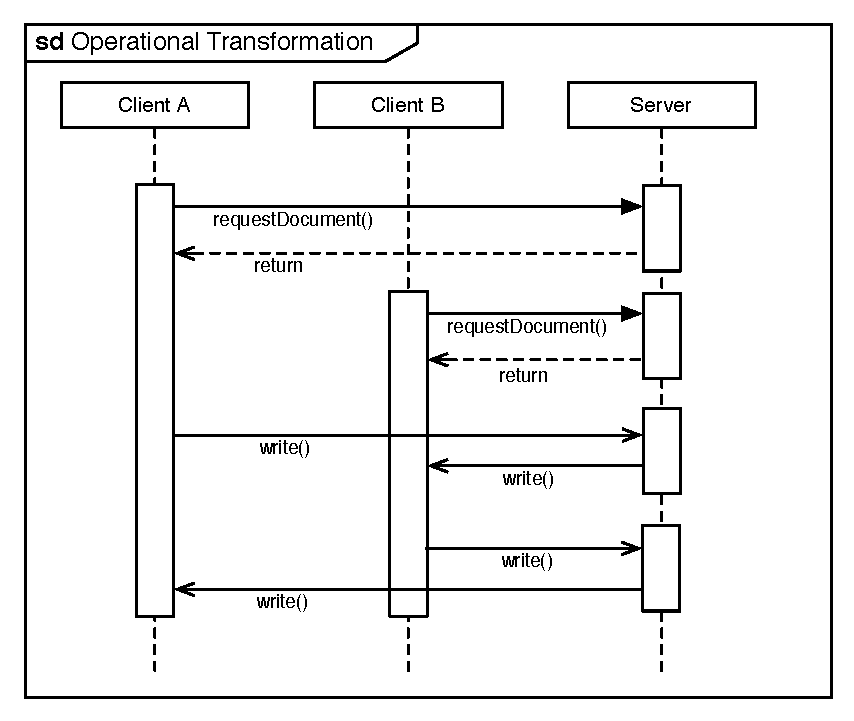
\includegraphics[width=0.5\textwidth]{ot_seq.pdf}
\caption{Sequence diagram of Operational Transformation}
\label{fig:optr}
\end{center}
\end{figure}

\textbf{Operational Transformation} (OT) is a class of algorithms that use event-passing to synchronize \cite{Ellis_1989}. Figure \ref{fig:optr} shows the interaction scheme of OT. All change events on the resource are captured and sent to the collaborating nodes. These change instructions are commonly known as patches. Eventual consistency\footnote{Eventual consistency describes that all accesses to a resource yield the same result when there have been not writes in a particular time span. \cite{Gustavsson_2002}} can be achieved through different models \cite{Sun_1998} \cite{Li_2004} \cite{Li_2005}. Google Docs\footnote{Google Docs, \url{https://docs.google.com/}, accessed 06/25/13} is a popular example application that uses OT.

\textbf{Differential Synchronization} is very similar to an event-passing approach \cite{Fraser_2009}. However, instead of capturing all changes as they happen, the change instructions are destilled by comparing two snapshots of the document. This approach is preferred when capturing all the user edits is a practical challenge.

Both Operational Transformation and Differential Synchronization support realtime collaboration. Even though concurrent editing of the same document is not a requirement, concurrent read access is (see: requirement \ref{req:concurrency}). Using automatic updates instead of manual ones greatly enhances the user experience. Both Operational Transformation and Differential Synchronization support realtime collaboration. Therefore, they are the best suited approaches for Project Zoom. Operational Transformation has been selected, because the system is already built using an event-based architecture in both the server \cite{Bocklisch_2013} and the client (see: section \ref{sec:eventbased}).

\subsection{Technology}
Because Project Zoom is a web application, the client code needs to be written in JavaScript\footnote{JavaScript is a scripting language that was designed for use in web browsers and was standarized under the name ECMAScript \url{http://www.ecma-international.org/publications/files/ECMA-ST/Ecma-262.pdf}.}. The presentation layer is built using the standard HTML\footnote{Hypertext Markup Language, \url{http://www.w3.org/TR/html5/}, accessed 06/19/13} and CSS\footnote{Cascading Style Sheets, \url{http://www.w3.org/TR/css-2010/}, accessed 06/19/13} technologies. The interactive graph relies on SVG\footnote{Scalable Vector Graphics, \url{http://www.w3.org/TR/SVG/}, accessed 06/19/13} because of its unique zooming and hit-test\footnote{Hit-testing is a technique to determine which user interface element intersects with the user's cursor \cite{Foley_1995}.} capabilities. The d3\footnote{Data-Driven Documents, \url{http://d3js.org/}, accessed 06/19/13} library is used to manipulate the SVG document.

\section{Model}

The Model is the component that is responsible for fetching the data from the server, listening on changes and passing changes back to the server. This section covers the techniques the client applies to handle the domain data on an abstract level. Bocklisch's thesis describes the actual domain data model in detail \cite{Bocklisch_2013}.

\subsection{Representing the data in the client application}

The data is represented through two container classes that wrap around the native objects of JavaScript: \texttt{DataItem} and \texttt{DataCollection}. Both classes extend the native objects with getter and setter methods for accessing and manipulating the respective properties or items. Using getters and setters is a popular technique of tracking changes in the data and emitting corresponding events \cite{Osmani_2013}. An alternative approach to container classes would be the \texttt{Object.observe} API \cite{Waldron_2012} which has yet to be standarized.

The container classes can be used to build hierarchical tree structures. In such a structure, property changes of child objects are then propagated to their ancestor objects. Also, nested properties can be accessed through the parent's \texttt{get} method using the JSON Pointer \footnote{RFC 6901, JavaScript Object Notation (JSON) Pointer, \url{http://tools.ietf.org/html/rfc6901}, accessed 06/20/13} syntax.

Both container classes provide methods for fetching data from the server. For that they use the XMLHttpRequest \cite{W3C_XHR} API of the browser. This technique is commonly referred to as Asynchronous JavaScript and XML (AJAX) \cite{Garrett_2005}. There is also support for \textit{lazy loading}\footnote{Lazy loading is a technique where data only is loaded once it is required instead of loading it upon initialization. \cite{Fowler_2002}} of properties or subtrees. When importing a native JavaScript object into an container properties with names starting with an underscore are treated as candidates for lazy loading. It is expected that their initial values contain information how to retrieve the data from the server (e.g. how to build the URL).

\subsection{Connecting to the server's REST interface}

\begin{figure}
\missingfigure{Object diagram}
\caption{Illustration of an example domain data structure.}
\label{fig:projectstruc}
\end{figure}

The server provides the data through an REST interface. Representational State Transfer (REST) is an architectural style on top of HTTP where resources are accessible through non-mutable URLs and are accessed and manipulated through the HTTP methods instead of custom URLs. \cite{Fielding_2000} 

The REST interface for Project Zoom relies on the JSON\footnote{RFC 4627,  The application/json Media Type for JavaScript Object Notation (JSON), \url{http://tools.ietf.org/html/rfc4627}, accessed 06/20/13} format for data exchange. As JSON is based on a subset of JavaScript, is is very easy to parse and create JSON documents through native APIs. The full specification of the project's REST interface is attached in the Appendix \ref{appendix:REST}.

Upon initialization the Model requests the \texttt{projects} and \texttt{tags} collections from the server. This is useful because all business logic depends on these data collections. Lazy loading would increase page loading time even further. As shown in figure \ref{fig:projectstruc} the projects collection is one of the root data structures in the system. % As shown in Appendix \ref{appendix:REST} the request \texttt{GET /projects} yields a list of project\todo{not clear which projects} objects that doesn't contain all properties in full detail. For example the \texttt{\_graphs} property is a lazy loading candidate that initially only holds the IDs of the referenced graphs. The Model loads the respective graph objects on-demand.


\subsection{Synchronizing changes with the server}

Changes to the server are transmitted using a patch-based format. Patches are documents that describe changes between two versions of a document. In many scenarios, patches have a substantially smaller footprint than their referenced document. Therefore, they are faster to send over a network. Furthermore, applying patches instead of replacing whole documents is less likely to cause consistency errors \cite{Ellis_1989}. Patches are also a key concept in Operational Transformation, which has been employed to support realtime collaboration.

Project Zoom uses the recently introduced JSON Patch standard \cite{RFC6902}. JSON Patch is a format for describing a list of mutations in an existing JSON document. A mutation entry contains an operation identifier, e.g. \texttt{add}, \texttt{remove} or \texttt{replace}, as well as a property address using the JSON Pointer syntax and a new value. Appendix \ref{appendix:JSONpatch} shows an example of a JSON patch applied to a JSON document. 
The JSON patches are generated by an accumulator object. It connects to a \texttt{DataItem} object and listens to the change events. Because \texttt{DataItem}s propagate change events from their child nodes, the accumulator can be attached to any node and will receive the change events from the complete subtree. For each change the accumulator appends a new patch entry to a list buffer, which will eventually be sent to the server.

For some user actions, e.g. dragging an element across the canvas, the amount of patch entries can grow very fast. To minimize the transportation footprint of the patches, the accumulator provides a method for compacting patches by reducing the amount of redundant entries in the patch. The proposed algorithm is shown in listing \ref{lst:patchcompact} and has a time complexity of $\mathcal O(n^2)$. Compacted patches are then sent to the server using the HTTP \texttt{PATCH} method.

\begin{figure}
\begin{lstlisting}[language=pseudo,caption={Pseudo code for compacting a chronologically ordered list of JSON patches},label={lst:patchcompact}]
foreach patch1, i in patches
  if patch1 is marked as overridden
    remove patch1
  
  foreach patch2, j in entries where i > j
    if patch2 removes the item or any parent of patch1
      remove patch1
      mark patch2 as overridden
      
    else if patch2 replaces the item of patch1 or any parent of patch1
      remove patch2
     
    else if patch2 replaces or removes a child item of patch1
      merge patch2 into patch1
      mark patch2 as overridden    
\end{lstlisting}
\end{figure}

The client is designed to listen for changes sent from the server. For that the client opens a WebSocket\footnote{WebSocket, \url{http://tools.ietf.org/html/rfc6455}, \url{http://www.w3.org/TR/2009/WD-websockets-20091222/}, both accessed 06/23/13} connection. The server sends JSON patches with an accompanying resource identifier, which get applied to the data structure in the client. Because of the event-driven architecture of the client, these changes will be propagated to the View immediately. As concurrent editing of a single resource (e.g. an interactive graph) is not a requirement (see: requirement \ref{req:concurrency}), conflicting edits will be rejected by the server.

\section{View}

The View is responsible for rendering the data to the user interface.

\subsection{Component interface}

\begin{wrapfigure}{R}{0.3\textwidth}
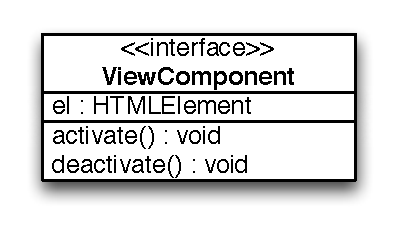
\includegraphics[width=0.3\textwidth]{viewinterface.pdf}
\caption{Class diagram of the View component interface}
\label{fig:viewinterface}
\end{wrapfigure}

The View is assembled by a hierarchical structure of View component instances. These instances share a common interface as shown in figure \ref{fig:viewinterface}. The View objects are responsible for controlling one element in the Document Object Model (DOM), which is referenced through the attribute \texttt{el}. At this stage the View component is not interactive yet. The method \texttt{activate} enables interactivity, by attaching event handlers to the DOM. \texttt{deactivate} then removes these event handlers, making the view component non-interactive again. This approach allows other components to control which View components are currently active. Consequently, parent components are responsible for activating and deactivation their children. The View components do not attach their element to the DOM themselves.

\subsection{Data integration}

Upon initialization View components are assigned with a \texttt{DataItem} or a \texttt{DataCollection}. The contained data is then used to render the user interface. Views tap into the event system and listen on changes from the Model to update accordingly. For example, when a user moves the cursor across the canvas to drag a graph node, the \texttt{position} property of the node is being altered by a controller (see: section \ref{sec:behavior}). This change is propagated to the view, which then renders the node at its new position. Server-sent changes are handled in the very same way. So, the view is agnostic to where the event originated.

\subsection{Architecture}

\begin{figure}
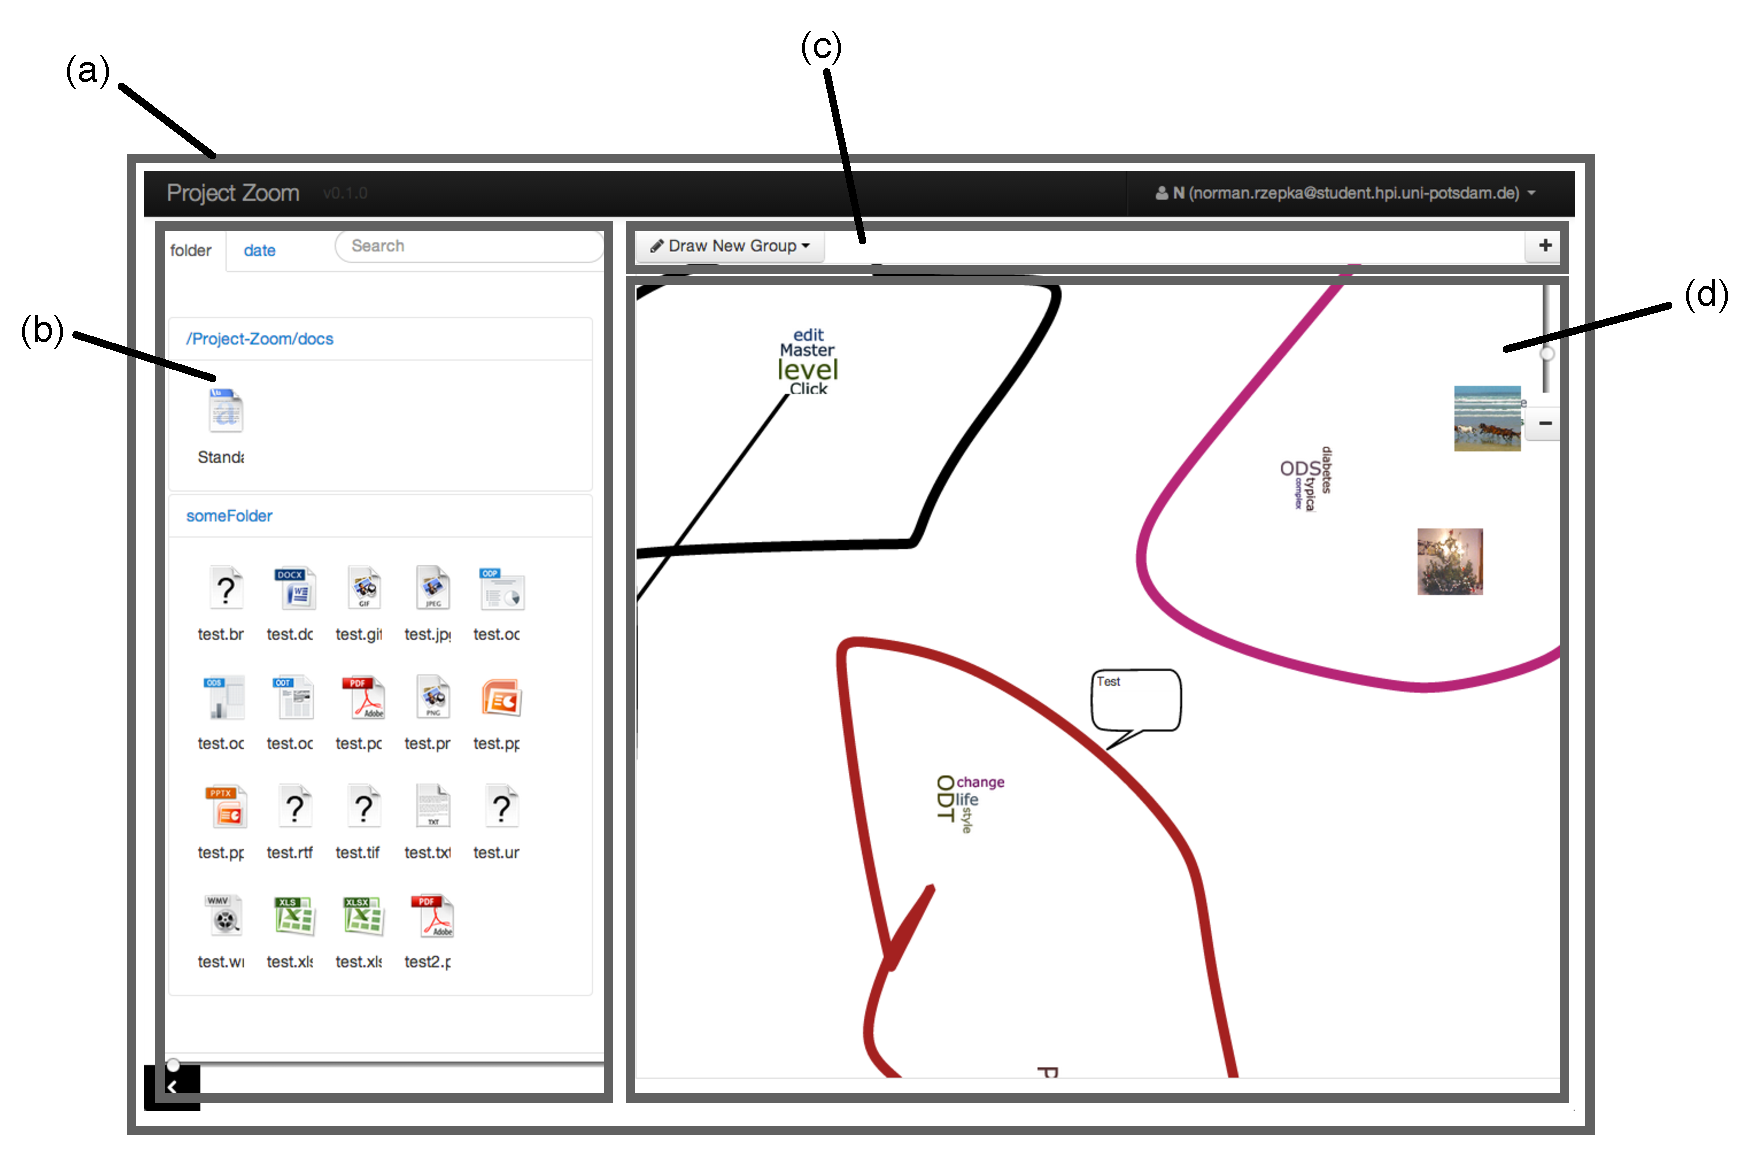
\includegraphics[width=\textwidth]{viewlayout.pdf}
\caption[Screenshot of the Process view with component annotations]{Screenshot of the Process view with component annotations: \textit{(a)} ProcessView, \textit{(b)} ArtifactFinder, \textit{(c)} Toolbar, \textit{(d)} Graph}
\label{fig:viewlayout}
\end{figure}

There are three main views: Overview view, Details view and Process view (see: section \ref{sec:design}). As shown in figure \ref{fig:arch} these are represented by three hierarchical View component structures. Figure \ref{fig:viewlayout} is an example of how the individual components have distributed responsibilities across the user interface.

\section{Controller}

The Controller components handle user interactions and manipulate the data in the Model as well as the Views.

\subsection{Main controller}
In Project Zoom, zooming is the main method for navigating from one view to another (see: section \ref{sec:design}). The main Controller handles this zoom-based behavior. For that the domain of zoom levels is split into several subranges as shown in figure \ref{fig:zoomtable}. The controller enforces states of the main views in each subrange as described.

The Controller works with the global range of zoom levels. This global zoom level is decoupled from the zoom level that the individual views work with. Because of this it is easier to alter the parameters in the controller while maintaining the assumptions in the view components and vice versa. The controller converts the global zoom level into the specific levels using pluggable functions.

\begin{figure}
\begin{center}
\begin{tabular}{|c|c|c|c|}
\hline
& Overview view & Details view & Process view \\ \hline
0-9 & active & - & - \\
10-19 & transition-out & transition-in & - \\
20-29 & - & active & - \\
30-39 & - & transition-out & transition-in \\
40-150 & - & - & active \\ \hline
\end{tabular}
\end{center}
\caption{Zoom level configurations}
\label{fig:zoomtable}
\end{figure}

\begin{wrapfigure}{R}{0.3\textwidth}
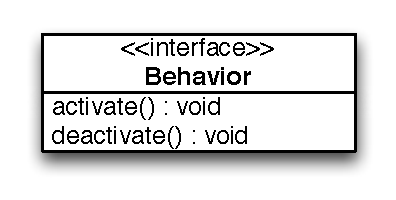
\includegraphics[width=0.3\textwidth]{behaviorinterface.pdf}
\caption{Class diagram of the Behavior interface}
\label{fig:behaviorinterface}
\end{wrapfigure}

\subsection{Behavior controllers}
\label{sec:behavior}

In addition to the main controller there are several other controllers that encapsulate a particular behavior in one of the main views, e.g. dragging nodes, drawing clusters or commenting. These behaviors share an interface as shown in figure \ref{fig:behaviorinterface}, which is similar to the interface of the View components . Again, the \texttt{activate} and \texttt{deactivate} methods enable or disable the interactivity provided by the respective behavior. Behaviors operate indepenently of each other and only communicate via events. For example, the deletion behavior emits an event whenever a node has been removed from the graph. The selection behavior recognizes this event and eliminates any references it had to that node. This loosely coupling makes it easy to extend the functionality of the application by adding custom behaviors. Behaviors alter the data in the Model. Because of the event-driven architecture these alterations are progated to update the View and sent to the server for persistence.

